\documentclass{article}

\usepackage{graphicx}
\usepackage{tikz}
\usepackage{tikzsymbols}
\usetikzlibrary{calc,patterns,shapes.geometric}
\pagestyle{empty}
\usepackage[margin=0pt]{geometry}
\geometry{papersize={14in,12in}}

\def\centerarc[#1](#2)(#3:#4:#5){\draw[#1] ($(#2)+({#5*cos(#3)},{#5*sin(#3)})$) arc (#3:#4:#5);}

\begin{document}
	\begin{figure}
		\centering
		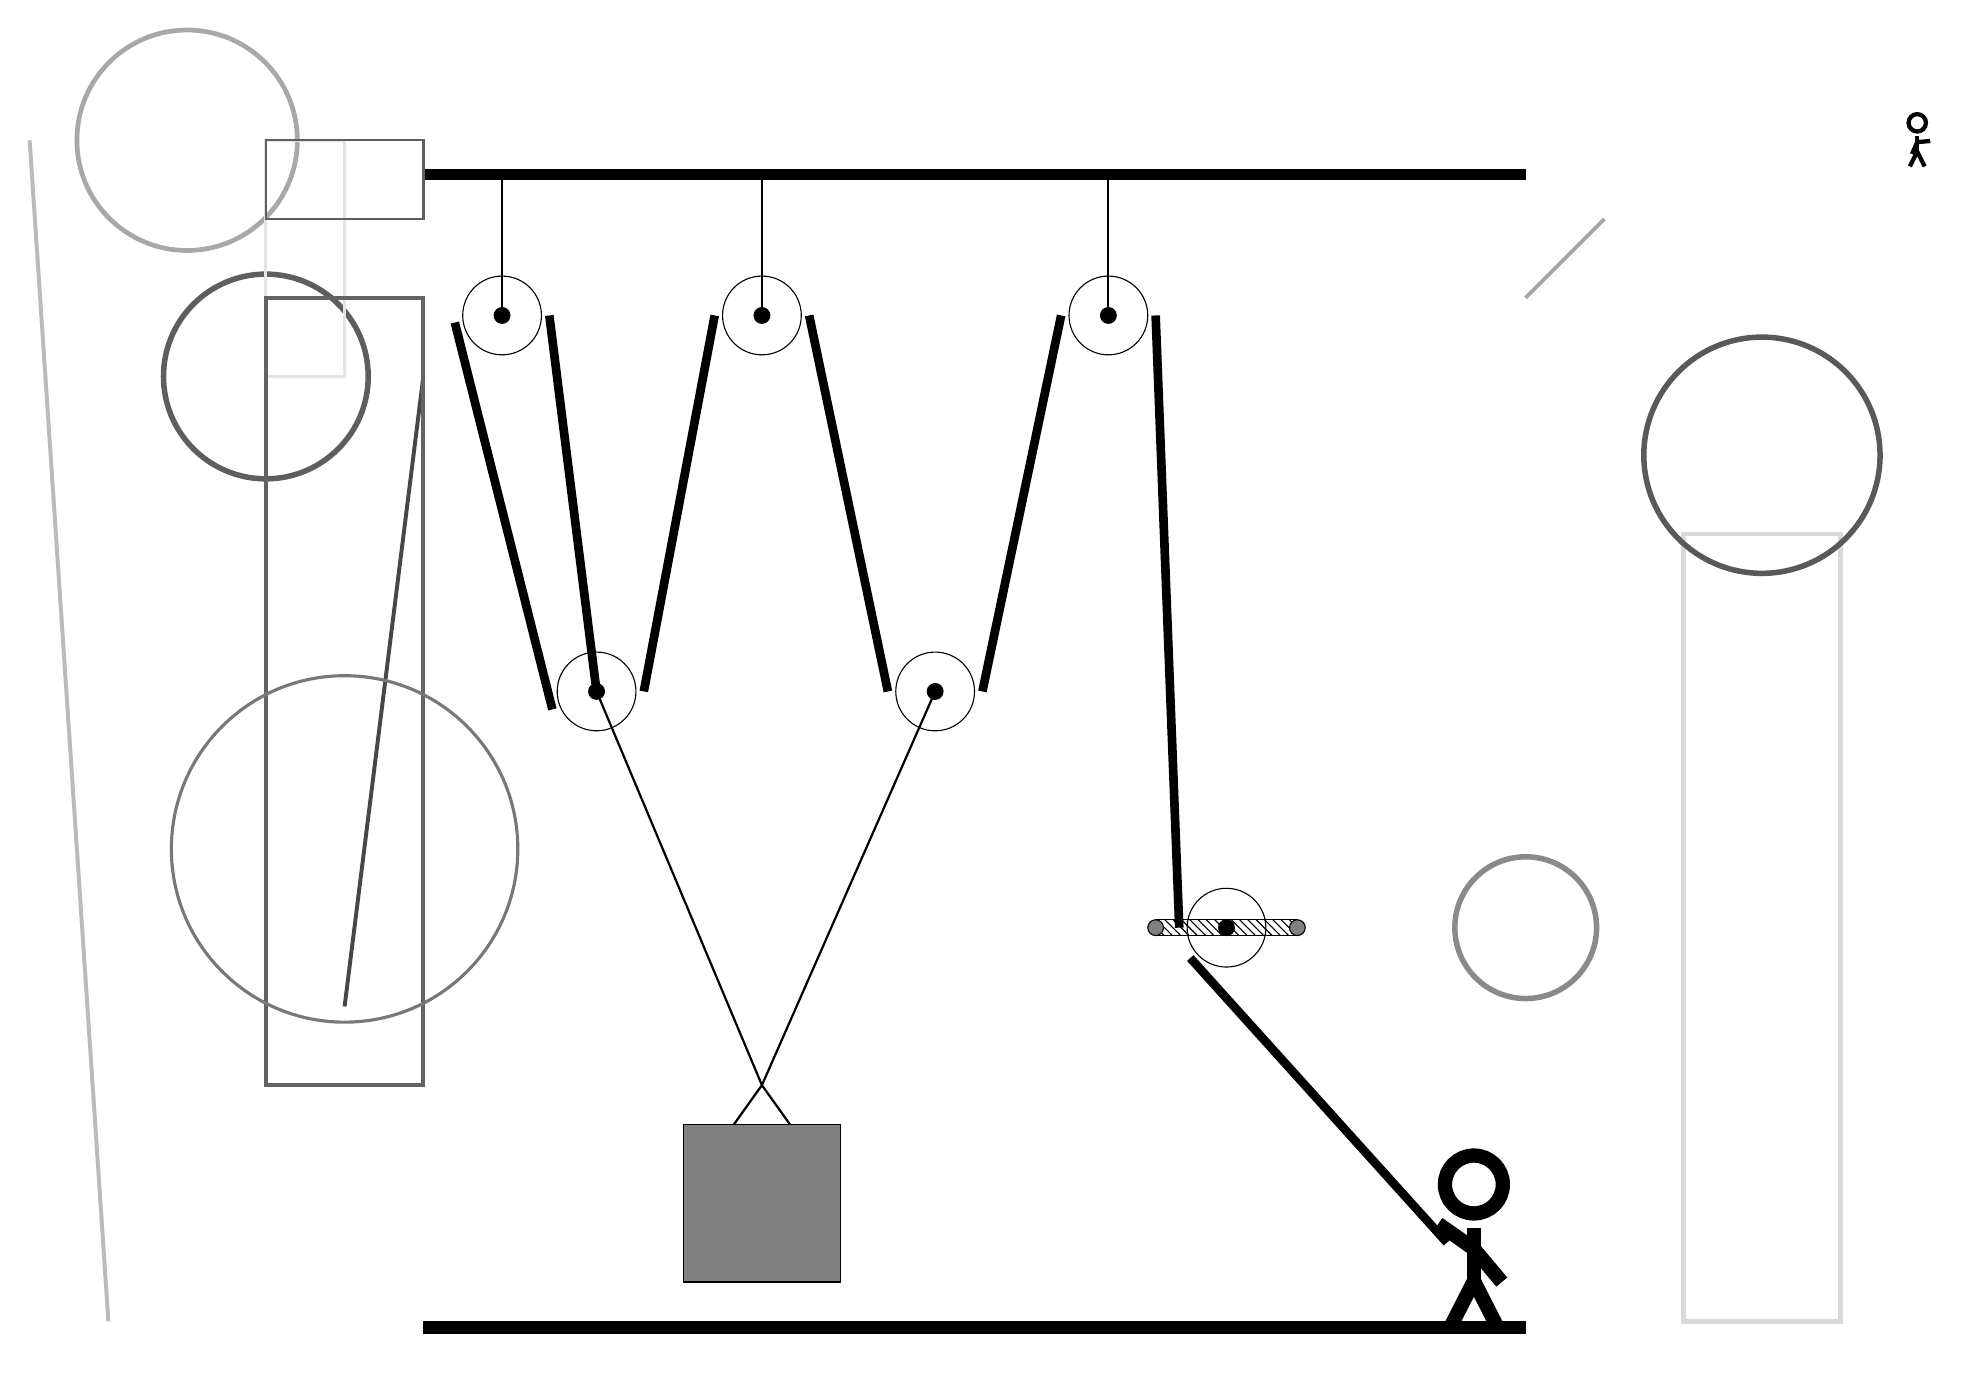
\begin{tikzpicture}
			%%%%% START %%%%%
			
			\draw[fill=black] (-2, 11.5) rectangle (12, 11.625);
			
			\draw (-1, 9.775) circle (0.5);
			\draw[fill=black] (-1, 9.775) circle (0.1);
			\draw[thick] (-1, 9.775) -- (-1, 11.5);
			
			\draw (2.3, 9.775) circle (0.5);
			\draw[fill=black] (2.3, 9.775) circle (0.1);
			\draw[thick] (2.3, 9.775) -- (2.3, 11.5);
			
			\draw (6.7, 9.775) circle (0.5);
			\draw[fill=black] (6.7, 9.775) circle (0.1);
			\draw[thick] (6.7, 9.775) -- (6.7, 11.5);
			
			\draw (0.2, 5) circle (0.5);
			\draw[fill=black] (0.2, 5) circle (0.1);
			
			\draw (4.5, 5) circle (0.5);
			\draw[fill=black] (4.5, 5) circle (0.1);
			
			\draw [line width=0.4mm, color=black!95](-6, 4) circle (0.0);
			
			\draw [line width=0.7mm, color=black!63](-4, 9) circle (1.3);
			\draw [line width=0.6mm, color=black!34](-5, 12) circle (1.4);
			\draw[line width=0.5mm, color=black!35](13, 11) -- (12, 10);
			\draw[line width=0.4mm, color=black!10] (-4, 12) rectangle (-3, 9);
			\draw[line width=0.3mm, color=black!63] (-2, 12) rectangle (-4, 11);
			\draw[line width=0.5mm, color=black!72](-3, 1) -- (-2, 9);
			\draw[line width=0.5mm, color=black!61] (-2, 10) rectangle (-4, 0);
			\draw [line width=0.7mm, color=black!46](12, 2) circle (0.9);
			
			\draw[line width=0.6mm, color=black!15] (14, -3) rectangle (16, 7);
			
			\node[line width=0.2mm, color=black!99] at (17, 12) {\Strichmaxerl[3][66][5]};
			
			\draw [line width=0.7mm, color=black!65](15, 8) circle (1.5);
			\draw [line width=0.4mm, color=black!53](-3, 3) circle (2.2);
			\draw[line width=0.5mm, color=black!27](-7, 12) -- (-6, -3);
			
			\draw (8.2, 2.0) circle (0.5);
			\draw[fill=black] (8.2, 2.0) circle (0.1);
			\draw[pattern=north west lines, pattern color=black] (7.3, 2.1) rectangle (9.1, 1.9);
			\draw[fill=black!50] (7.3, 2.0) circle (0.1);
			\draw[fill=black!50] (9.1, 2.0) circle (0.1);
			
			\draw[thick] (0.2, 5) -- (2.3, 0)  -- (4.5, 5);
			\draw[thick]  (1.8, -0.7) -- (2.3, 0) -- (2.8, -0.7);
			\draw[fill=black!50] (1.3, -0.5) rectangle (3.3, -2.5);
			
			\draw[line width=1.1mm] (0.2, 5) -- (-0.4, 9.775);
			\centerarc[line width=1.1mm](-1, 9.775)(0:200:0.6);
			\draw[line width=1.1mm] (-1.6, 9.685) -- (-0.361, 4.772);
			\centerarc[line width=1.1mm](0.2, 5)(200:360:0.6);
			\draw[line width=1.1mm](0.8, 5) -- (1.7, 9.775);
			\centerarc[line width=1.1mm](2.3, 9.775)(0:180:0.6);
			\draw[line width=1.1mm] (2.9, 9.775) -- (3.9, 5);
			\centerarc[line width=1.1mm](4.5, 5)(180:360:0.6);
			\draw[line width=1.1mm] (5.1, 5) -- (6.1, 9.775);
			\centerarc[line width=1.1mm](6.7, 9.775)(0:180:0.6);
			\draw[line width=1.1mm](7.3, 9.775) --  (7.6, 2.0);
			\centerarc[line width=1.1mm](8.2, 2.0)(180:220:0.6);
			\draw[line width=1.1mm](7.7404, 1.6143) -- (11, -2);
			
			\node at (11.3, -2) {\Strichmaxerl[10][-35][-50]};
			
			\draw[fill=black] (-2, -3) rectangle (12, -3.15);
			
			%%%%% END %%%%%
		\end{tikzpicture}
	\end{figure}	
\end{document}